\documentclass[a4paper,12pt]{article}

% --- Packages ---
\usepackage[utf8]{inputenc}
\usepackage[T1]{fontenc}
\usepackage[english]{babel}
\usepackage{graphicx}
\usepackage{amsmath, amssymb}
\usepackage{hyperref}
\usepackage{natbib}
\usepackage{geometry}
\geometry{margin=2.5cm}

% --- Title Info ---
\title{Praktikum Data Science: Phase 1 Report}
\author{Éva Mária Szabó \\ \small Karlsruher Institut für Technologie (KIT)}
\date{\today}

\begin{document}

% --- Title Page ---
\maketitle
\tableofcontents
\newpage

% --- Sections ---
\section{Introduction}
In my team, which is Team 3, we did most parts of our exercise in a pair programming style. Due to that, most commits are not under my name, since I was not the one who pushed them. However, I still contributed significantly to the project, so I will summarize my contributions here.

\section{Week 1 - Data Exploration}
To kick things off, I created some bar charts and pie charts based on the data.
\begin{figure}[h]
    \centering
    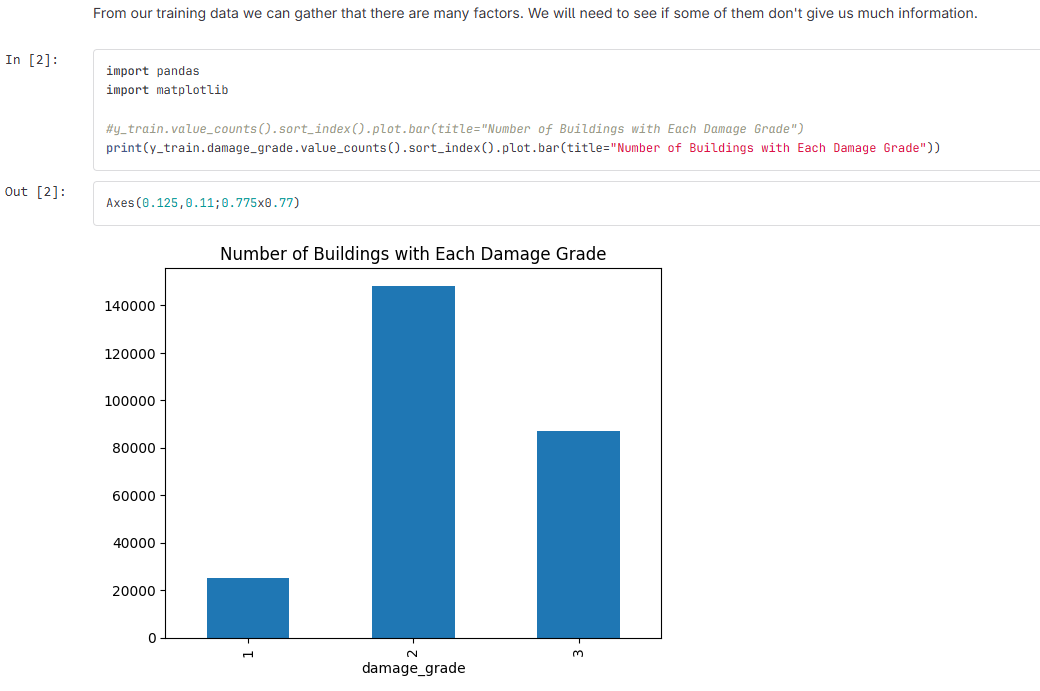
\includegraphics[width=0.8\textwidth]{figures/example_plot_jupyter.png}
    \caption{Example of a plot I created in Jupyter Notebook}
    \label{fig:data_exploration}
\end{figure}
In Figure~\ref{fig:data_exploration}, you can see an example of a plot I created in Jupyter Notebook. This helped us better understand the data and identify potential issues.  
I also wrote some initial code to load the data and perform basic statistical analysis, which was crucial for our understanding of the dataset. Additionally, I commented on each plot and the conclusions we drew from them.

\section{Week 2 - Cleaning and Pipeline}
From this week onwards, I was mostly responsible for research. For this week, that meant looking into how to clean the data and how to set up a pipeline for our data processing. I found that we could use the \texttt{sklearn} library for this purpose, which is very powerful and flexible.  
I also wrote some initial code to clean the data and build a pipeline structure. Since I had previously worked on some data science projects, I was able to apply my knowledge and experience to this project, such as how to handle missing values, encode categorical variables, and scale numerical features.

For this week's presentation, although it was not my turn, I helped Nimród with the slides and provided feedback on the content. I also created some plots to visualize the data cleaning process and the pipeline structure.

\section{Week 3 - Feature Engineering}
We had many discussions about which features to use and how to create new ones. I researched various feature engineering techniques, such as one-hot encoding, label encoding, and feature scaling. We also decided to create some new columns based on my idea of using volume percentage instead of height and area percentages.

\section{Week 4 - Prediction Models}
Since we agreed that I would be giving the presentation for this week, I focused on understanding different prediction models. I researched various algorithms such as logistic regression, decision trees, random forests, etc.  
This helped us understand the strengths and weaknesses of each model and how to choose the best one for our dataset. I also wrote some initial code to evaluate the models and compare their performance.

\section{Week 5 - Dealing with Imbalanced Multi-Class Data}
I researched various techniques for dealing with imbalanced multi-class data, such as oversampling, undersampling, threshold tuning, and using different evaluation metrics. I also implemented some of these techniques in Python using the \texttt{sklearn} library.  
This helped us understand how to handle imbalanced data and how to choose the best evaluation metric for our dataset.

\section{Week 6 - Hyperparameter Tuning}
For this week, it was Ádám's turn to present, so he did most of the work. However, I continued my research on cross-validation and different prediction models. I also helped him prepare the presentation and provided feedback on his slides, as well as created some plots to visualize the results of the hyperparameter tuning process.

\section{Conclusion}
In conclusion, I contributed significantly to the project by researching various topics, implementing code, and preparing presentations. I learned a lot about data science and how to apply it to real-world problems. I also enjoyed working in a team and collaborating with my teammates. I hope that my contributions will help us achieve our goals and successfully complete the project.

% --- Bibliography ---
%\bibliographystyle{plainnat}
%\bibliography{mybib}

\end{document}
